\section{Dirichlet Evolution}
\label{dirichlet_triangle_evolution}

Our goal is to model the evolution of a distribution on a probability simplex. Fig.\ \ref{fig:kitchen_uncertainty} shows this for two classes. In general, we can do the same for multiple classes. Fig.\ \ref{fig:dirichlet_triangle_evolution} shows an example of the  Dirichlet distribution for three classes, and how it changes over time. This evolution is the output of the \DirModel model trained on the 3-G dataset, created to simulate the car example from Sec.\ \ref{introduction} (see also Fig.\ \ref{fig:car_categorical} in Appendix \ref{datasets}). The three classes: \textit{overtaking}, \textit{breaking} and \textit{collision} occur independently of each other at three different times. The represent the corners of the triangle in Fig.~\ref{fig:dirichlet_triangle_evolution}.

We can distinguish three cases: (a) at first we are certain that the most likely class is \textit{overtaking}; (b) as time passes, the most likely class becomes \textit{breaking}, (c) and finally \textit{collision}. After that, we are in the area where we have not seen any data and do not have a confident prediction (d).

\begin{figure}[H]
\centering
    \begin{subfigure}{0.25\textwidth}
        \centering
        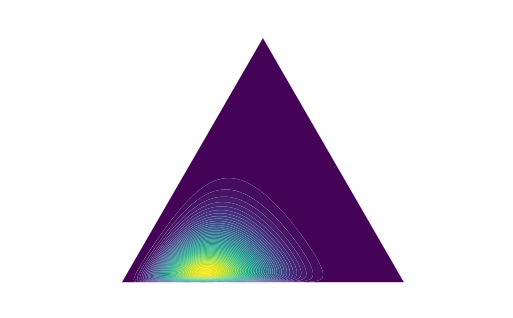
\includegraphics[width=\linewidth]{images/0.png}
        \caption{$\DeltaTime = 0$}
    \end{subfigure}
    \hspace{-0.4cm}
    \begin{subfigure}{0.25\textwidth}
        \centering
        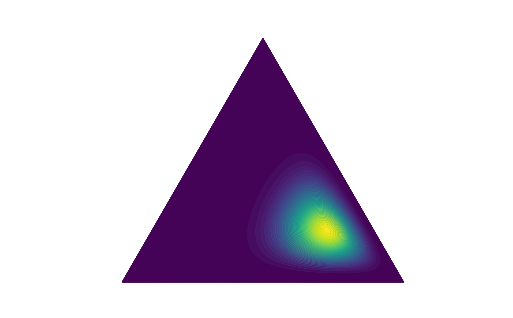
\includegraphics[width=\linewidth]{images/13.png}
        \caption{$\DeltaTime = 0.5$}
    \end{subfigure}
    \hspace{-0.4cm}
    \begin{subfigure}{0.25\textwidth}
        \centering
        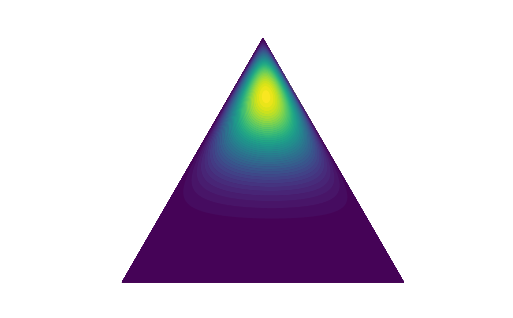
\includegraphics[width=\linewidth]{images/33.png}
        \caption{$\DeltaTime = 1.$}
    \end{subfigure}
    \hspace{-0.4cm}
    \begin{subfigure}{0.25\textwidth}
        \centering
        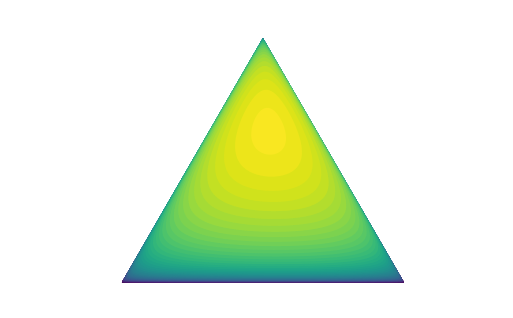
\includegraphics[width=\linewidth]{images/60.png}
		\caption{$\DeltaTime = 2.$}
    \end{subfigure}
    \caption{Dirichlet distribution at different time  for the 3-G dataset with $\sigma =1.$}
    \label{fig:dirichlet_triangle_evolution}
\end{figure}